% Compile with XeLaTeX or Tectonic. Times New Roman must be installed.
\documentclass[11pt,letterpaper]{article}
\usepackage{fontspec}
\IfFileExists{fonts/TNR-Regular.ttf}{%
  \setmainfont{TNR-Regular.ttf}[Path=fonts/,BoldFont=TNR-Bold.ttf,ItalicFont=TNR-Italic.ttf,BoldItalicFont=TNR-BoldItalic.ttf]
  \setsansfont{TNR-Regular.ttf}[Path=fonts/,BoldFont=TNR-Bold.ttf,ItalicFont=TNR-Italic.ttf,BoldItalicFont=TNR-BoldItalic.ttf]
  \setmonofont{TNR-Regular.ttf}[Path=fonts/]
}{%
  \setmainfont{Times New Roman}
  \setsansfont{Times New Roman}
  \setmonofont{Times New Roman}
}
\usepackage[italic]{mathastext}

\usepackage[margin=.82in,top=.78in,bottom=.78in]{geometry}
\usepackage{microtype}
\usepackage{setspace}
\setstretch{1.08}
\usepackage[table]{xcolor}
\usepackage{array,longtable,tabularx,booktabs}
\usepackage{graphicx,float,caption}
\usepackage{enumitem}
\usepackage{titlesec}
\usepackage{fancyhdr}
\usepackage{hyperref}
\hypersetup{hidelinks,pdftitle={Limits of REDD-Only Evidence for NILM Deployment},pdfauthor={Stephen Makonin}}
\urlstyle{same}
\Urlmuskip=0mu plus 1mu
\usepackage{pgfplots}
\pgfplotsset{compat=1.18}
\definecolor{EvidenceBlue}{HTML}{305F82}
\definecolor{EvidenceGold}{HTML}{B89850}
\definecolor{EvidenceGray}{HTML}{D4D8DB}
\pgfplotsset{whitepaper/.style={width=\linewidth,height=3.6in,
  tick label style={font=\small},label style={font=\small},
  xticklabel={\pgfmathprintnumber[assume math mode=true]{\tick}},
  yticklabel={\pgfmathprintnumber[assume math mode=true]{\tick}},
  legend style={font=\small,draw=none,fill=none},legend cell align=left,
  axis line style={black!65},tick style={black!65},
  grid style={black!12},ymajorgrids=true,
  scaled y ticks=false,scaled x ticks=false,
  /pgf/number format/1000 sep={,}}}

\definecolor{RuleGray}{HTML}{D9D9D9}
\definecolor{HeaderGray}{HTML}{E9EDF0}
\arrayrulecolor{RuleGray}
\renewcommand{\arraystretch}{1.18}
\setlength{\parindent}{0pt}
\setlength{\parskip}{6pt}
\setlength{\headheight}{14pt}
\pagestyle{fancy}
\fancyhf{}
\fancyhead[R]{\small REDD and NILM experimental validation}
\fancyfoot[C]{\small Page \thepage}
\renewcommand{\headrulewidth}{0pt}
\renewcommand{\footrulewidth}{0pt}
\titleformat{\section}{\large\bfseries}{\thesection}{.6em}{}
\titlespacing*{\section}{0pt}{14pt}{7pt}
\captionsetup{font=small,labelfont=bf,justification=raggedright,singlelinecheck=false}
\setlist[itemize]{leftmargin=1.2em,itemsep=4pt,topsep=4pt}
\setlength{\emergencystretch}{2em}
\widowpenalty=10000
\clubpenalty=10000
\begin{document}
{\LARGE\bfseries Limits of REDD-Only Evidence for NILM Deployment\par}
\vspace{6pt}
{\large Measurement context, preprocessing, and complementary validation\par}
\vspace{5pt}
Stephen Makonin\quad Companion technical note, version 1.1\\
25 October 2026
\vspace{7pt}

\section*{Purpose and scope}
REDD helped establish open energy-disaggregation research and remains valuable for historical reproduction, benchmark comparisons, and focused algorithmic tests. Its contribution should be distinguished from the limits of any particular evaluation that uses it. This note concerns the additional evidence needed when a REDD result is used to support deployment across households, seasons, or measurement systems. \cite{ref1}

High accuracy on a disclosed REDD subset can support a well-defined benchmark result. Broader claims require evidence suited to the intended operating conditions. The conventional low-frequency release has limited household and temporal coverage, different nominal sampling intervals for mains and circuit measurements, documented gaps, and questions about measurement compatibility. These properties make data preparation part of the experiment; reporting that preparation helps readers interpret and reproduce the score. \cite{ref1,ref2,ref3}

Preprocessing deserves particular attention when an experiment fills or deletes missing readings, presents resampled labels as higher-resolution observations, or replaces measured mains using target submeters. Such choices can change test difficulty as well as measured algorithm performance. The historical importer examined here is Stephen Makonin's own software: its exclusion and repair rules are not REDD's original acquisition pipeline or a standard REDD preprocessing prescription. \cite{ref4,ref5}

We recommend retaining REDD as a historical comparison and diagnostic dataset while requiring independent validation on complementary datasets. AMPds2 and R1Hz provide longitudinal energy tests, with R1Hz adding one-second electrical streams; UK-DALE provides documented calibration of selected whole-house meters; REFIT adds household and usage diversity; and RAE offers useful circuit measurements when the provenance of its aggregate is checked. Each has limitations. No dataset name is a substitute for an audit of the actual channels and intervals used. \cite{ref7,ref8,ref9,ref10,ref13}

REDD-only evidence should be interpreted within its disclosed homes, intervals, measurements, and processing rules. Data limitations can raise or lower measured performance; they do not establish that a particular published result is incorrect. The questions are which task was tested, how much valid evidence remained, and whether a claimed advantage transfers to independent measurement conditions.

This technical note combines published dataset descriptions and diagnostic studies with an analysis of the archived DataWrangle\_REDD code and log. No fresh raw-archive replay or NILM model experiment is reported. Historical log counts describe that software pipeline; illustrative calculations are not REDD measurements. The current Python 3 importer preserves measured mains and exports observation masks; the archived repair counts do not describe its behavior.

\textbf{Author disclosure.} Stephen Makonin wrote the historical importer examined here and coauthored the AMPds2, RAE, and R1Hz dataset publications. Recommendations identify complementary evaluation roles and do not rank these datasets as universally more accurate. The same measurement, missingness, provenance, and reporting requirements apply to every dataset. \cite{ref7,ref10,ref13}

\section{What the REDD benchmark actually contains}
REDD was an important contribution to open energy-disaggregation research. Its original system combined high-frequency whole-house waveforms with lower-rate circuit and plug measurements. The detailed hardware description reports circuit polling at approximately three seconds and whole-house waveforms at 15 kHz. Processed whole-house power is available at nominally one-second intervals. REDD therefore cannot accurately be described as having uniformly synchronized one-hertz appliance ground truth. \cite{ref1,ref2}

The conventional public low-frequency release contains six homes. The original 2011 paper described ten monitored homes and 119 combined days at the time of writing; those collection figures must not be interpreted as 119 days for each released home. Usable duration also depends on the selected channels and the definition of a gap. The NILMTK diagnostic study reports a house-level median mains uptime of 18 days, with a range of 4 to 19 days under its procedure. These are diagnostic results, not universal durations for every REDD export. \cite{ref1,ref2}

A calendar span is not the same as valid evaluation exposure. A file can begin in April and end in May while containing long outages, short dropouts, and intervals with no usable target measurement. Intersecting mains with several targets can leave less data than any channel alone. Researchers should report the calendar span, observed duration, valid shared duration, and appliance activation counts separately.

Nor is every labeled circuit an individual appliance. A kitchen-outlet or lighting circuit may combine several devices. Recovering that circuit is a legitimate task, but a circuit-level score does not demonstrate recognition of each appliance connected to it. The original REDD descriptions and experiments include such grouped loads. \cite{ref1}

These limitations matter because a small set of repeated operating cycles can contain many correlated samples. Thousands of overlapping windows from one refrigerator are not thousands of independent tests of household generalization. Short records also provide little evidence about seasons, appliance replacement, changing occupancy, and rare operational states. Those are limits on the conclusions an experiment can support, even when its numerical score is computed correctly.

\section{Timing and missing readings change the experiment}
Different sampling cadences, unequal recording boundaries, and true clock errors are separate problems. A UTC timestamp alone does not prove that two meters integrate power over the same physical interval. The INDiC study notes that REDD house 2 appliance recording began about six hours after mains recording. That is evidence of different recording boundaries, not evidence of a universal six-hour clock offset. The official NILMTK converter also sorts REDD records because the raw data is not always ordered. \cite{ref3,ref6}

Joining channels by row number is invalid when timestamps differ. Nearest-neighbor joins, forward filling, interpolation, and bin averaging each impose different assumptions about when a measurement applies. Repeating a three-second appliance observation onto a one-second grid increases the number of labels; it does not create three independent one-second observations. Transition times remain uncertain at the native measurement scale.

A simple calculation shows why this matters. Consider a constructed 1 kW rectangular activation lasting 120 seconds. An otherwise exact prediction shifted by four seconds has 8,000 watt-seconds of absolute error, or 2.22 Wh. Its samplewise ON-state F1 is about 0.967 on an otherwise OFF background. For an activation lasting only ten seconds, the same shift reduces that samplewise F1 to 0.60. These are illustrative timing effects, not an estimate of REDD clock error. An algorithm can be penalized by uncertain ground truth, while a generous matching tolerance can conceal the same uncertainty.

Missing readings are independently documented. NILMTK illustrates extended mains outages and recurring circuit dropouts. Its published REDD diagnostics report a median 10 percent dropout rate when long gaps are excluded and a median 40 percent mains uptime relative to the relevant recording span. Both quantities depend on the diagnostic definitions and channels; neither should be advertised as a universal REDD missingness rate. \cite{ref2}

Zero filling asserts that an unobserved appliance was off. Forward filling asserts that its previous state persisted. Linear interpolation can invent a gradual transition. Dropping rows can remove difficult intervals; treating the retained rows as contiguous can join events that were hours apart. Event pairers, recurrent models, and duration-based classifiers are especially sensitive to these changes. The direction of bias is conditional: corrupted labels can depress performance, whereas selective exclusion or smoothing can make a task easier.

Preserve observation masks and original timestamps, split sequences at excluded gaps, and document model-state handling. Report excluded observed target energy and activation counts; energy during absent-reference periods remains unknown unless estimated explicitly. Imputed values may support inference but should not silently become measured ground truth.

\section{A historical importer case study}
This section examines Stephen Makonin's own DataWrangle\_REDD importer at commit 66ea7e0, dated 30 July 2015. Its grid, grouping, exclusion, and negative-residual repair rules are design choices of that historical software, rather than attributes of REDD's acquisition system. The code places observations on an integer-second grid, groups channels, skips rows without a mains timestamp or acceptable grouped fields, and attempts to repair negative aggregate residuals. The archived import log is a record of this preparation attempt. \cite{ref4,ref5}

\begingroup\small\setlength{\tabcolsep}{4pt}
\begin{longtable}{|>{\centering\arraybackslash}p{0.467in}|>{\centering\arraybackslash}p{1.305in}|>{\centering\arraybackslash}p{1.022in}|>{\centering\arraybackslash}p{0.798in}|>{\centering\arraybackslash}p{1.509in}|>{\centering\arraybackslash}p{1.032in}|}
\caption{Historical export counts recorded in DataWrangle\_REDD}\\
\hline\rowcolor{HeaderGray}
\textbf{House} & \textbf{One second grid positions} & \textbf{Exported rows} & \textbf{Retained percent} & \textbf{Lead and lag substitutions} & \textbf{Residual rebuilds}\\\hline
\endfirsthead
\hline\rowcolor{HeaderGray}
\textbf{House} & \textbf{One second grid positions} & \textbf{Exported rows} & \textbf{Retained percent} & \textbf{Lead and lag substitutions} & \textbf{Residual rebuilds}\\\hline
\endhead
1 & 3,134,094 & 406,748 & 12.98 & 450 & 74\\\hline
2 & 3,026,450 & 316,840 & 10.47 & 249 & 25\\\hline
3 & 3,870,508 & 376,150 & 9.72 & 906 & 156\\\hline
4 & 4,145,367 & 428,076 & 10.33 & 427 & 78\\\hline
5 & 3,786,978 & 77,451 & 2.05 & 163 & 19\\\hline
6 & 2,022,746 & 192,192 & 9.50 & 187 & 124\\\hline
\end{longtable}
\endgroup
Retained percent is exported rows divided by the log’s dense one-second grid length. Lead and lag substitutions combine two counters in the log; residual rebuilds correspond to its negative-noise counter. These are pipeline counts, not independently verified clock faults, sensor failure rates, continuous recording days, or model scores. \cite{ref5}

The denominator is essential. Much of the grid has no exact circuit observation because the native circuit cadence is approximately three seconds; outages and nonmatching availability remove further rows. Thus the reported 87 to 98 percent shrinkage must not be relabeled as 87 to 98 percent sensor data loss. Completeness is also checked after channel grouping, so a passing row does not establish that every original constituent channel was present. \cite{ref4,ref5}

The log names its exports with a 3sec suffix while the inspected script uses lowf. It is therefore an archived processing record rather than proof that this exact script version produced every logged result. A fresh audit would require the raw files, checksums, and executed configuration. What the archive establishes is narrower but consequential: the final evaluation sample is heavily determined by joining, grouping, exclusion, and repair rules.

\section{Repair can compromise the independence of a test}
The historical DataWrangle\_REDD snapshot can change measured mains using submeter information. When summed submeter measurements exceed the mains reading, the script attempts to search neighboring mains at nominal offsets of one through nine seconds and substitutes a value that makes the residual nonnegative. If that search fails, it rebuilds mains from the target sum plus an estimated residual. This describes a heuristic in the archived code, not a verified timing correction or REDD's acquisition procedure. The operations are visible in lines 129 to 163 of the pinned script. \cite{ref4}

This approach may help investigate inconsistent records, but it cannot independently prove the physical cause of a negative residual. The condition can reflect timing differences, incompatible electrical quantities, meter error, channel mapping, or incomplete measurement definitions. A successful substitution is a successful heuristic repair, not an independently measured clock correction. For example, the log records an imported mains value of 172 and grouped submeter sum of 1,801 at timestamp 1303207434, followed by a replacement mains value of 1,837. This establishes an imbalance in the imported representation, without isolating its physical cause. \cite{ref5}

For blind NILM evaluation, the methodological consequence is that information from the target measurements can determine the input presented to the model. Rebuilding aggregate input from the same submeters used as ground truth introduces a dependence that an ordinary deployed system does not have. Searching future mains values also uses evidence unavailable at the original timestamp. Such a track should be disclosed as retrospective, target-informed repair, with results reported separately from tests on independently measured mains.

The archive is valuable because it makes its transformations inspectable. The log records 2,858 mains substitutions or rebuilds across 1,797,457 exported rows, approximately 0.159 percent. These sparse row counts do not establish that repair explains a large performance improvement; the impact depends on event location and the energy affected. This case study does not establish that any particular REDD publication used this repository or these repair rules.

The broader issue also arises when researchers construct an aggregate by summing selected targets. A controlled aggregate can test source separation under known conditions, but it removes unmonitored loads and couples the input to its labels. Klemenjak, Makonin, and Elmenreich found that testing on denoised aggregates usually improved performance in their study, with exceptions. Their results do not imply a universal inflation factor or a simple monotonic relationship between residual magnitude and difficulty. \cite{ref11}

A strong paper therefore reports two clearly identified tracks where useful: independently measured mains for deployment-oriented evidence, and constructed or repaired aggregates for controlled analysis. It preserves raw observations and publishes the locations of every input change, whether target labels influenced that change, and whether the operation requires future data.

\section{Measurement compatibility and the meaning of ground truth}
Low sampling rate and inaccurate measurement are not synonyms. A well-calibrated one-minute meter may provide reliable energy measurements while missing switching detail. A high-rate stream may preserve transitions while suffering calibration or timing errors. A dataset comparison must distinguish electrical accuracy, temporal resolution, synchronization, completeness, and population coverage.

Electrical quantity is particularly important. NILMTK conventionally maps REDD mains channels to apparent power and circuit channels to active power. Its metadata acknowledges inconsistent source documentation about the circuit meter. Researchers should therefore verify the convention used in their actual files rather than assert that every REDD export has a metrologically established active-versus-apparent mismatch. \cite{ref3}

Active power P, measured in watts, and apparent power S, measured in volt-amperes, cannot simply be substituted for one another in an additive energy model. If mains and target measurements are incompatible, the residual between mains and the sum of targets is not a clean measure of unknown appliances. Even with compatible units, that residual can include timing error, incomplete circuit coverage, double counting, and meter error. Its sign and magnitude require diagnosis.

For this reason, an experiment should identify both split-phase mains channels, its channel aggregation rules, the measurement type of each stream, and any voltage or power-factor assumptions. A balance check should be run on valid aligned intervals and should retain negative residuals as diagnostic evidence rather than automatically forcing them to zero.

Ground truth also has a scope. A metered circuit is a reference for that circuit; it is not necessarily a reference for each device on it. An interpolated appliance trace is a reconstruction; it is not a new physical observation. A cluster assigned an appliance name after comparison with test labels demonstrates clustering agreement under that mapping rule. It does not by itself demonstrate autonomous appliance identification.

The recommendation is to choose complementary reference data by the property being tested. Measurement quality should support energy-error claims. Timing and native sampling should support event claims. Independent homes and longer records should support generalization claims. All three are needed when a system is presented as ready for practical deployment.

\section{Complementary datasets and evaluation roles}
The following comparison uses associated journal descriptions, supplemented by the author-maintained R1Hz technical documentation. It identifies useful evidence for different evaluation purposes, without a universal accuracy ranking. The author's involvement in AMPds2, RAE, and R1Hz is disclosed above; their own coverage and recovery limits remain part of the comparison. Each actual release requires a version and quality audit. \cite{ref7,ref8,ref9,ref10,ref12,ref13}

\begingroup\small\setlength{\tabcolsep}{4pt}
\begin{longtable}{|>{\centering\arraybackslash}p{0.924in}|>{\raggedright\arraybackslash}p{2.925in}|>{\raggedright\arraybackslash}p{2.617in}|}
\caption{Dataset selection by the property requiring validation}\\
\hline\rowcolor{HeaderGray}
\textbf{Dataset} & \textbf{Contribution to validation} & \textbf{Limit that must remain visible}\\\hline
\endfirsthead
\hline\rowcolor{HeaderGray}
\textbf{Dataset} & \textbf{Contribution to validation} & \textbf{Limit that must remain visible}\\\hline
\endhead
AMPds2 \cite{ref7} & One Canadian home over 730 days at one-minute intervals. Industrial DENT meters have specified 1 percent accuracy and less than 0.5 percent typical error. Useful for longitudinal energy and multistate-load tests. & One home limits population inference. One-minute readings cannot resolve fast events. Timestamp corrections and filled readings must be accounted for.\\\hline
R1Hz \cite{ref13} & A 757-day calendar span at one Burnaby, Canada dwelling, with five aligned one-hertz electrical streams, 19 logical channels, interval-energy products, utility comparisons, and retained acquisition records. Useful for longitudinal energy and temporal-resolution tests. & One dwelling and mixed circuits limit generalization. Retain all quality markers, including s and +; exclude imputed references from primary ground-truth scoring or assess them separately. Calendar coverage is not uninterrupted observation.\\\hline
UK-DALE \cite{ref8} & Five homes. Houses 1, 2 and 5 add one-hertz active-power mains and 16 kHz waveforms. Selected mains systems were individually calibrated; a resistive-load test reported less than 2 percent relative error. & The reference meter also has uncertainty. Appliance observations are approximately six seconds apart, and coverage is incomplete. Mains calibration does not validate every target meter.\\\hline
REFIT \cite{ref9} & Twenty homes over approximately two years, with aggregate and nine selected appliance streams per home at eight-second intervals. Useful for household diversity and unknown-load robustness. & A breadth test, not a precision reference. Its paper documents current-only measurement, asynchronous readings, outages, and imputation.\\\hline
RAE \cite{ref10} & The original two-home release includes up to 24 circuits at one hertz for 72 and 59 days, plus independent utility observations at roughly eight to fifteen seconds. & The one-hertz mains column can be calculated from submeters or separately measured. Metadata must identify which; constructed and measured aggregates need separate evaluation tracks.\\\hline
IDEAL \cite{ref12} & A larger optional robustness test. The study includes 255 homes; an enhanced subset of 39 adds selected appliance and active-power monitoring. & Appliance ground truth is not available for all 255 homes. Missingness and the difference between ordinary and enhanced instrumentation require subset-specific auditing.\\\hline
\end{longtable}
\endgroup
AMPds2 and R1Hz are useful complementary choices for longitudinal energy evaluation. AMPds2 cannot establish second-level latency; R1Hz adds one-second measurements over a longer calendar span but requires explicit handling of recovered intervals. Neither single-home dataset establishes population generalization. UK-DALE supports selected calibrated-mains comparisons, with appliance timing still requiring attention. REFIT tests more homes and unmonitored loads, while introducing its own data-quality constraints. RAE requires a distinction between measured and calculated aggregate channels. These roles are complementary.

\section{A minimum standard for credible NILM experiments}
We recommend the following requirements for papers making broad claims about NILM accuracy, generalization, or real-time use. These are proposed evaluation requirements, not claims that an existing dataset satisfies them automatically.

\textbf{Identify the physical test signal.} Publish the dataset release, raw-file checksums, home and channel identifiers, electrical quantities and units, selected dates, and whether the aggregate is independently measured, reconstructed, or target-informed. Record the software revision and complete configuration.

\textbf{Publish a data-quality audit.} Report native sample-interval distributions, duplicates, ordering faults, outages, short-dropout rates, and valid shared exposure. Supply masks for observed, imputed, excluded, and repaired values. Give valid duration, activation counts, and target energy by home and appliance; document every exclusion.

\textbf{Freeze the preprocessing and split rules.} Estimate any alignment correction or calibration on designated training or calibration intervals, then freeze it before testing. State interpolation limits and bin boundaries. Split sequences at gaps and prevent overlapping windows or complete activations from crossing train, validation, and test boundaries.

\textbf{Test independent homes and datasets.} Separate same-home chronological testing from held-out-home testing. Keep test labels out of model selection and input repair. Add a dataset chosen for measurement quality and another chosen for household diversity or realistic unmonitored loads. Report failures as well as pooled averages.

\textbf{Match resolution without inventing observations.} Report native-resolution performance and a common-resolution comparison where appropriate. Use a documented downsampling rule that respects measured intervals. Do not represent upsampled ground truth as new temporal evidence or claim an event timestamp more precise than the reference supports.

\textbf{Evaluate on shared valid intervals.} Apply the same predeclared observation masks to every algorithm. Score imputed or repaired regions separately. Pair power MAE with energy error, activation precision and recall, and complete per-appliance results. Include simple zero-output, constant-output, and feature-matched baselines where appropriate.

\textbf{Measure when predictions become available.} Log the first causal prediction and each later revision. Include observation, settling, window, and cycle-completion delays in reported latency. A model that identifies an activation after switch-off should be assessed for that completed-cycle task, not credited with immediate switch-on identification.

\textbf{Make the statistical unit explicit.} Estimate household-level uncertainty for new-household claims. Use nested temporal or activation blocks for within-household repeatability, preserving dependence. Do not treat densely sampled points or overlapping windows as independent replicates. Report sensitivity to gap thresholds, alignment tolerances, preprocessing, and important parameter choices.

\section{How reviewers should interpret REDD results}
A reproducible REDD result can support a limited algorithmic claim: the method performs as stated on the disclosed channels, time periods, electrical quantities, and quality masks. A study of a controlled constructed aggregate can support a source-separation claim under those construction assumptions. Neither result alone establishes generalization across acquisition systems or the wider household population.

A deployment-oriented claim requires more. The result should survive a second measurement system, a broader set of homes or operating conditions, explicit gap handling, and an evaluation of output availability. High accuracy on one or two familiar REDD homes should therefore prompt scrutiny of data preparation and task definition before it is credited as evidence of a broadly superior NILM system.

Reviewers should request clarification when a paper describes all REDD streams as one hertz, omits the usable shared duration, gives no policy for missing readings, confuses circuit labels with appliances, or reports noise ratios without checking compatible measurements. Claims of real-time use also require the observation delay, while claims of autonomous appliance recognition require a documented label-mapping procedure.

The same standards must apply to alternatives. A longer or newer dataset can still contain imputed values, asynchronous meters, uncertain units, and incomplete appliance coverage. It is the combination of transparent measurements, reproducible processing, appropriate claims, and independent tests that makes the evidence credible.

REDD continues to support historical reproduction and targeted algorithmic evaluation. When claims extend to practical operation across households or measurement systems, researchers should show data integrity and test the claimed advantage under complementary conditions. Transparent processing and evidence proportionate to the claim allow subsequent work to build on REDD's contribution.

\clearpage
\section{Quantitative selection through the archived pipeline}
The additional analysis parses all six house summaries and all 476 detailed fallback pairs in the archived log. Counts reconcile within each house: no-timestamp rows plus incomplete grouped rows plus exported rows equal the dense grid length. Every detailed fallback pair matches its house counter and its printed residual arithmetic. This is a reproducible analysis of a historical log, not a new ingestion of raw REDD.~\cite{ref5}
\begin{figure}[H]
\centering
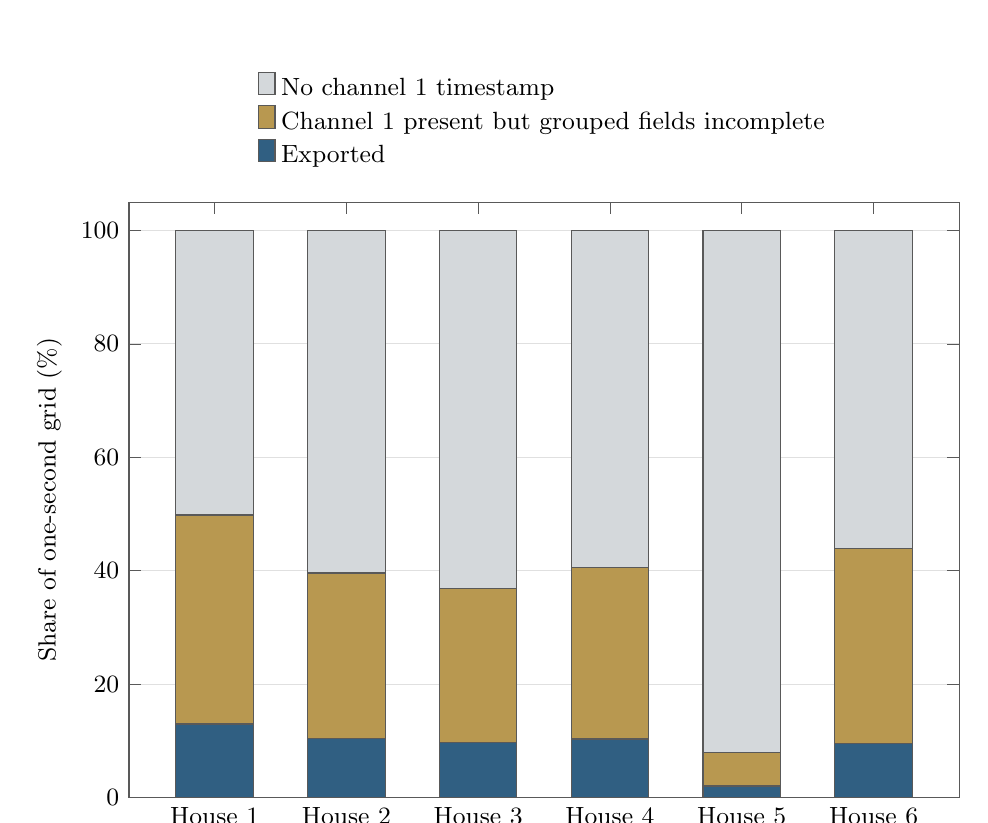
\begin{tikzpicture}
\begin{axis}[whitepaper,ybar stacked,bar width=28pt,
  ymin=0,ymax=105,xmin=.35,xmax=6.65,
  xtick={1,2,3,4,5,6},xticklabels={House 1,House 2,House 3,House 4,House 5,House 6},
  ytick={0,20,40,60,80,100},ylabel={Share of one-second grid (\%)},
  legend columns=1,legend style={at={(.5,1.04)},anchor=south},
  reverse legend=true]
\addplot[fill=EvidenceBlue,draw=black!65] coordinates {(1,12.97816849) (2,10.46903137) (3,9.71836255) (4,10.32661282) (5,2.04519276) (6,9.50153900)};
\addlegendentry{Exported}
\addplot[fill=EvidenceGold,draw=black!65] coordinates {(1,36.84994770) (2,29.13294454) (3,27.15752041) (4,30.19667499) (5,5.93272525) (6,34.37233345)};
\addlegendentry{Channel 1 present but grouped fields incomplete}
\addplot[fill=EvidenceGray,draw=black!65] coordinates {(1,50.17188380) (2,60.39802409) (3,63.12411704) (4,59.47671219) (5,92.02208199) (6,56.12612755)};
\addlegendentry{No channel 1 timestamp}
\end{axis}
\end{tikzpicture}

\caption{Disposition of integer-second grid positions in the archived import. Categories are mutually exclusive and sum to 100 percent. The incomplete category includes intentional native submeter cadence as well as unavailable or nonmatching fields; the log cannot separate those causes. These shares are not sensor-loss rates. Source: archived DataWrangle\_REDD log.~\cite{ref5}}
\end{figure}

\begingroup\small\setlength{\tabcolsep}{4pt}
\begin{longtable}{|>{\centering\arraybackslash}p{0.555in}|>{\centering\arraybackslash}p{1.211in}|>{\centering\arraybackslash}p{2.270in}|>{\centering\arraybackslash}p{2.320in}|}
\caption{Denominators that must not be confused}\\
\hline\rowcolor{HeaderGray}
\textbf{House} & \textbf{Calendar grid days} & \textbf{Channel 1 rows per grid percent} & \textbf{Exported per channel 1 rows percent}\\\hline
\endfirsthead
\hline\rowcolor{HeaderGray}
\textbf{House} & \textbf{Calendar grid days} & \textbf{Channel 1 rows per grid percent} & \textbf{Exported per channel 1 rows percent}\\\hline
\endhead
1 & 36.27 & 49.83 & 26.05\\\hline
2 & 35.03 & 39.60 & 26.44\\\hline
3 & 44.80 & 36.88 & 26.35\\\hline
4 & 47.98 & 40.52 & 25.48\\\hline
5 & 43.83 & 7.98 & 25.64\\\hline
6 & 23.41 & 43.87 & 21.66\\\hline
\end{longtable}
\endgroup
Pooled across houses, 7,056,896 channel-1 records occupy 35.31 percent of 19,986,143 grid positions. The 1,797,457 exported rows represent 8.99 percent of that grid, or 25.47 percent of observed channel-1 rows. These are different denominators. Grid days are first-to-last timestamp spans, not continuous uptime; channel 1 alone does not certify that both mains legs are present.

\clearpage
\section{Frequency of recorded input changes}
The archived counters identify 1,381 lead substitutions, 1,001 lag substitutions, and 476 fallback rebuilds. Together these are 2,858 edits across 1,797,457 exported rows: 0.1590 percent, or 15.90 per 10,000. The labels describe heuristic operations rather than independently measured clock errors.~\cite{ref4,ref5}
\begin{figure}[H]
\centering
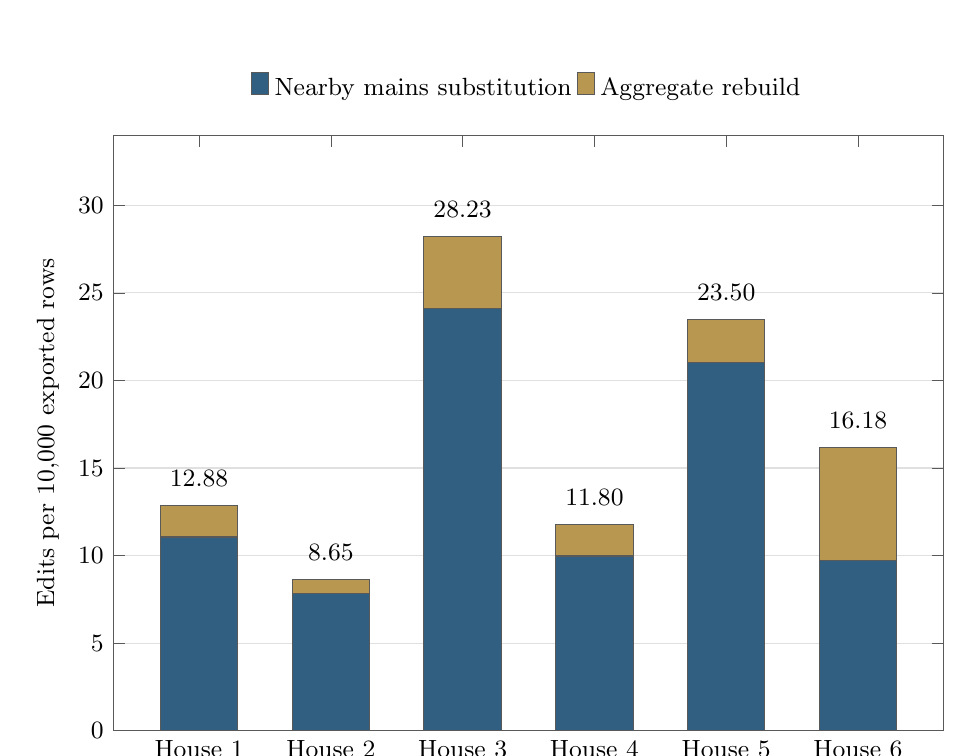
\begin{tikzpicture}
\begin{axis}[whitepaper,ybar stacked,bar width=28pt,
  ymin=0,ymax=34,xmin=.35,xmax=6.65,
  xtick={1,2,3,4,5,6},xticklabels={House 1,House 2,House 3,House 4,House 5,House 6},
  ylabel={Edits per 10,000 exported rows},
  legend columns=2,legend style={at={(.5,1.04)},anchor=south}]
\addplot[fill=EvidenceBlue,draw=black!65] coordinates {(1,11.06336110) (2,7.85885621) (3,24.08613585) (4,9.97486428) (5,21.04556429) (6,9.72985348)};
\addlegendentry{Nearby mains substitution}
\addplot[fill=EvidenceGold,draw=black!65] coordinates {(1,1.81930827) (2,0.78904179) (3,4.14728167) (4,1.82210635) (5,2.45316394) (6,6.45188145)};
\addlegendentry{Aggregate rebuild}
\node[font=\small,anchor=south] at (axis cs:1,13.382669367765793){12.88};
\node[font=\small,anchor=south] at (axis cs:2,9.147897992677692){8.65};
\node[font=\small,anchor=south] at (axis cs:3,28.73341751960654){28.23};
\node[font=\small,anchor=south] at (axis cs:4,12.29697063138321){11.80};
\node[font=\small,anchor=south] at (axis cs:5,23.99872822817007){23.50};
\node[font=\small,anchor=south] at (axis cs:6,16.681734931734933){16.18};
\end{axis}
\end{tikzpicture}

\caption{Recorded edits per 10,000 exported rows. Nearby mains substitutions combine the historical lead and lag counters; rebuilds use the negative-noise counter. Labels show total edits per 10,000. Normalization permits comparison of unequal exported row counts, but does not make the houses independent samples of a population. Source: archived DataWrangle\_REDD log.~\cite{ref5}}
\end{figure}
The rates range from 8.65 per 10,000 exported rows in house 2 to 28.23 in house 3. Fallback rebuilds alone account for 0.02648 percent of all exported rows. The archive does not record the magnitude of every nearby-value substitution, so the next distribution applies only to the fallback subset.

The sparse frequency is an important limit on the criticism: these counts do not establish that repair dominates a complete test or explains any particular NILM score. Conversely, a small row share does not guarantee a small event or energy effect. A transition can be influential even when it occupies few timestamps. Measuring the effect on model performance would require the raw and repaired series, identical evaluation masks, and a controlled comparison.

\clearpage
\section{Magnitude of the detailed fallback rebuilds}
Each of the 476 paired fallback records increases the imported mains value. The pooled median increase is 301, the mean is 624.07, the 90th percentile is 1,772.5, and the maximum is 5,116. Values remain in the archive's integer power units; the export filename says VA, but this analysis does not independently establish the measurand or calibration.~\cite{ref5}
\begin{figure}[H]
\centering
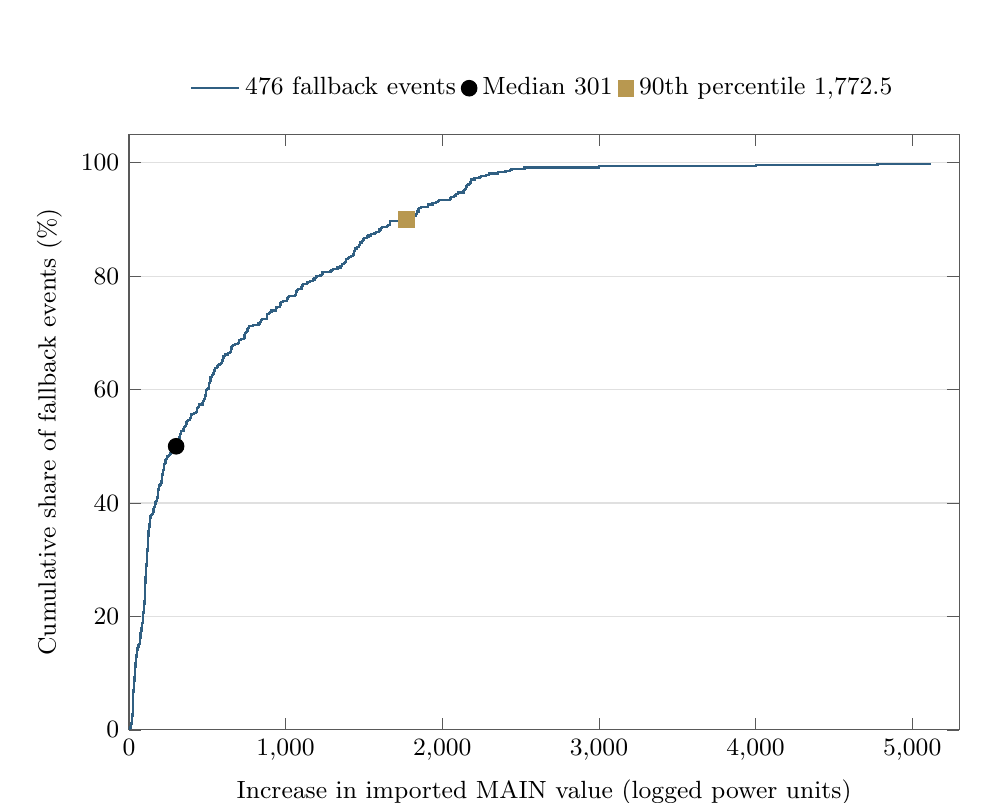
\begin{tikzpicture}
\begin{axis}[whitepaper,xmin=0,xmax=5300,ymin=0,ymax=105,
  xtick={0,1000,2000,3000,4000,5000},ytick={0,20,40,60,80,100},
  xlabel={Increase in imported MAIN value (logged power units)},
  ylabel={Cumulative share of fallback events (\%)},
  legend columns=3,legend style={at={(.5,1.04)},anchor=south}]
\addplot[EvidenceBlue,thick,const plot] coordinates {(0,0) (3,0.21008403) (7,0.42016807) (12,0.63025210) (12,0.84033613) (15,1.05042017) (16,1.26050420) (17,1.47058824) (17,1.68067227) (17,1.89075630) (18,2.10084034) (19,2.31092437) (21,2.52100840) (22,2.73109244) (24,2.94117647) (25,3.15126050) (25,3.36134454) (25,3.57142857) (25,3.78151261) (25,3.99159664) (25,4.20168067) (25,4.41176471) (26,4.62184874) (27,4.83193277) (27,5.04201681) (27,5.25210084) (27,5.46218487) (27,5.67226891) (28,5.88235294) (28,6.09243697) (28,6.30252101) (28,6.51260504) (28,6.72268908) (29,6.93277311) (30,7.14285714) (31,7.35294118) (31,7.56302521) (31,7.77310924) (32,7.98319328) (32,8.19327731) (32,8.40336134) (34,8.61344538) (35,8.82352941) (35,9.03361345) (35,9.24369748) (36,9.45378151) (37,9.66386555) (37,9.87394958) (37,10.08403361) (39,10.29411765) (39,10.50420168) (39,10.71428571) (40,10.92436975) (40,11.13445378) (41,11.34453782) (41,11.55462185) (41,11.76470588) (44,11.97478992) (45,12.18487395) (46,12.39495798) (46,12.60504202) (46,12.81512605) (48,13.02521008) (48,13.23529412) (50,13.44537815) (50,13.65546218) (51,13.86554622) (51,14.07563025) (54,14.28571429) (55,14.49579832) (57,14.70588235) (61,14.91596639) (66,15.12605042) (68,15.33613445) (69,15.54621849) (70,15.75630252) (71,15.96638655) (71,16.17647059) (73,16.38655462) (73,16.59663866) (74,16.80672269) (74,17.01680672) (75,17.22689076) (79,17.43697479) (80,17.64705882) (80,17.85714286) (82,18.06722689) (82,18.27731092) (82,18.48739496) (85,18.69747899) (85,18.90756303) (88,19.11764706) (88,19.32773109) (89,19.53781513) (89,19.74789916) (89,19.95798319) (91,20.16806723) (92,20.37815126) (92,20.58823529) (93,20.79831933) (94,21.00840336) (94,21.21848739) (95,21.42857143) (96,21.63865546) (97,21.84873950) (97,22.05882353) (98,22.26890756) (99,22.47899160) (99,22.68907563) (100,22.89915966) (100,23.10924370) (101,23.31932773) (101,23.52941176) (101,23.73949580) (101,23.94957983) (102,24.15966387) (103,24.36974790) (103,24.57983193) (103,24.78991597) (104,25.00000000) (104,25.21008403) (104,25.42016807) (104,25.63025210) (104,25.84033613) (106,26.05042017) (106,26.26050420) (106,26.47058824) (106,26.68067227) (106,26.89075630) (108,27.10084034) (109,27.31092437) (109,27.52100840) (109,27.73109244) (109,27.94117647) (110,28.15126050) (110,28.36134454) (110,28.57142857) (111,28.78151261) (111,28.99159664) (112,29.20168067) (113,29.41176471) (113,29.62184874) (113,29.83193277) (113,30.04201681) (114,30.25210084) (115,30.46218487) (115,30.67226891) (115,30.88235294) (115,31.09243697) (116,31.30252101) (117,31.51260504) (118,31.72268908) (118,31.93277311) (119,32.14285714) (119,32.35294118) (119,32.56302521) (120,32.77310924) (120,32.98319328) (120,33.19327731) (120,33.40336134) (121,33.61344538) (121,33.82352941) (123,34.03361345) (123,34.24369748) (124,34.45378151) (124,34.66386555) (125,34.87394958) (125,35.08403361) (126,35.29411765) (126,35.50420168) (127,35.71428571) (131,35.92436975) (131,36.13445378) (131,36.34453782) (133,36.55462185) (133,36.76470588) (133,36.97478992) (135,37.18487395) (135,37.39495798) (138,37.60504202) (140,37.81512605) (146,38.02521008) (151,38.23529412) (153,38.44537815) (156,38.65546218) (156,38.86554622) (159,39.07563025) (160,39.28571429) (164,39.49579832) (165,39.70588235) (168,39.91596639) (169,40.12605042) (173,40.33613445) (177,40.54621849) (177,40.75630252) (177,40.96638655) (183,41.17647059) (183,41.38655462) (185,41.59663866) (186,41.80672269) (186,42.01680672) (187,42.22689076) (189,42.43697479) (191,42.64705882) (191,42.85714286) (192,43.06722689) (199,43.27731092) (205,43.48739496) (208,43.69747899) (208,43.90756303) (209,44.11764706) (210,44.32773109) (210,44.53781513) (211,44.74789916) (213,44.95798319) (214,45.16806723) (218,45.37815126) (218,45.58823529) (218,45.79831933) (223,46.00840336) (223,46.21848739) (224,46.42857143) (225,46.63865546) (226,46.84873950) (232,47.05882353) (233,47.26890756) (233,47.47899160) (235,47.68907563) (244,47.89915966) (244,48.10924370) (246,48.31932773) (255,48.52941176) (261,48.73949580) (267,48.94957983) (277,49.15966387) (288,49.36974790) (291,49.57983193) (295,49.78991597) (298,50.00000000) (304,50.21008403) (304,50.42016807) (305,50.63025210) (310,50.84033613) (312,51.05042017) (319,51.26050420) (320,51.47058824) (322,51.68067227) (324,51.89075630) (327,52.10084034) (332,52.31092437) (332,52.52100840) (334,52.73109244) (348,52.94117647) (349,53.15126050) (351,53.36134454) (359,53.57142857) (362,53.78151261) (365,53.99159664) (367,54.20168067) (369,54.41176471) (375,54.62184874) (389,54.83193277) (391,55.04201681) (395,55.25210084) (396,55.46218487) (399,55.67226891) (417,55.88235294) (427,56.09243697) (433,56.30252101) (434,56.51260504) (435,56.72268908) (441,56.93277311) (448,57.14285714) (449,57.35294118) (469,57.56302521) (472,57.77310924) (474,57.98319328) (477,58.19327731) (479,58.40336134) (484,58.61344538) (485,58.82352941) (489,59.03361345) (490,59.24369748) (491,59.45378151) (493,59.66386555) (494,59.87394958) (496,60.08403361) (507,60.29411765) (509,60.50420168) (512,60.71428571) (512,60.92436975) (513,61.13445378) (517,61.34453782) (518,61.55462185) (520,61.76470588) (521,61.97478992) (521,62.18487395) (531,62.39495798) (532,62.60504202) (535,62.81512605) (544,63.02521008) (545,63.23529412) (546,63.44537815) (548,63.65546218) (549,63.86554622) (560,64.07563025) (566,64.28571429) (578,64.49579832) (589,64.70588235) (594,64.91596639) (596,65.12605042) (598,65.33613445) (598,65.54621849) (604,65.75630252) (604,65.96638655) (612,66.17647059) (634,66.38655462) (645,66.59663866) (649,66.80672269) (650,67.01680672) (651,67.22689076) (654,67.43697479) (656,67.64705882) (665,67.85714286) (676,68.06722689) (697,68.27731092) (701,68.48739496) (701,68.69747899) (717,68.90756303) (733,69.11764706) (738,69.32773109) (738,69.53781513) (741,69.74789916) (743,69.95798319) (748,70.16806723) (751,70.37815126) (756,70.58823529) (760,70.79831933) (765,71.00840336) (768,71.21848739) (791,71.42857143) (827,71.63865546) (836,71.84873950) (842,72.05882353) (843,72.26890756) (850,72.47899160) (879,72.68907563) (880,72.89915966) (882,73.10924370) (883,73.31932773) (895,73.52941176) (901,73.73949580) (910,73.94957983) (938,74.15966387) (938,74.36974790) (942,74.57983193) (965,74.78991597) (965,75.00000000) (967,75.21008403) (969,75.42016807) (981,75.63025210) (1009,75.84033613) (1010,76.05042017) (1017,76.26050420) (1020,76.47058824) (1061,76.68067227) (1065,76.89075630) (1066,77.10084034) (1066,77.31092437) (1073,77.52100840) (1077,77.73109244) (1101,77.94117647) (1102,78.15126050) (1107,78.36134454) (1113,78.57142857) (1134,78.78151261) (1139,78.99159664) (1158,79.20168067) (1173,79.41176471) (1185,79.62184874) (1192,79.83193277) (1197,80.04201681) (1222,80.25210084) (1231,80.46218487) (1236,80.67226891) (1287,80.88235294) (1293,81.09243697) (1301,81.30252101) (1331,81.51260504) (1350,81.72268908) (1360,81.93277311) (1360,82.14285714) (1374,82.35294118) (1381,82.56302521) (1383,82.77310924) (1383,82.98319328) (1400,83.19327731) (1404,83.40336134) (1416,83.61344538) (1430,83.82352941) (1434,84.03361345) (1435,84.24369748) (1438,84.45378151) (1442,84.66386555) (1445,84.87394958) (1454,85.08403361) (1466,85.29411765) (1468,85.50420168) (1473,85.71428571) (1476,85.92436975) (1489,86.13445378) (1492,86.34453782) (1497,86.55462185) (1498,86.76470588) (1522,86.97478992) (1529,87.18487395) (1545,87.39495798) (1568,87.60504202) (1577,87.81512605) (1596,88.02521008) (1599,88.23529412) (1610,88.44537815) (1616,88.65546218) (1646,88.86554622) (1653,89.07563025) (1665,89.28571429) (1667,89.49579832) (1668,89.70588235) (1770,89.91596639) (1775,90.12605042) (1802,90.33613445) (1807,90.54621849) (1832,90.75630252) (1834,90.96638655) (1838,91.17647059) (1840,91.38655462) (1848,91.59663866) (1848,91.80672269) (1849,92.01680672) (1864,92.22689076) (1907,92.43697479) (1910,92.64705882) (1938,92.85714286) (1958,93.06722689) (1974,93.27731092) (1979,93.48739496) (2051,93.69747899) (2054,93.90756303) (2077,94.11764706) (2084,94.32773109) (2087,94.53781513) (2098,94.74789916) (2135,94.95798319) (2141,95.16806723) (2144,95.37815126) (2149,95.58823529) (2154,95.79831933) (2160,96.00840336) (2167,96.21848739) (2176,96.42857143) (2180,96.63865546) (2182,96.84873950) (2185,97.05882353) (2206,97.26890756) (2238,97.47899160) (2249,97.68907563) (2279,97.89915966) (2299,98.10924370) (2357,98.31932773) (2404,98.52941176) (2432,98.73949580) (2442,98.94957983) (2525,99.15966387) (3002,99.36974790) (4005,99.57983193) (4779,99.78991597) (5116,100.00000000)};
\addlegendentry{476 fallback events}
\addplot[only marks,mark=*,mark size=2.8pt,black] coordinates {(301,50)};
\addlegendentry{Median 301}
\addplot[only marks,mark=square*,mark size=2.8pt,EvidenceGold] coordinates {(1772.5,90)};
\addlegendentry{90th percentile 1,772.5}
\end{axis}
\end{tikzpicture}

\caption{Empirical cumulative distribution of MAIN after minus MAIN before for the 476 detailed fallback events. Quantiles use linear interpolation at zero-based rank (n - 1)p. This selected subset contains negative-residual cases that reached the rebuild branch; it is not a distribution of all REDD errors or all 2,858 edits. Source: paired historical log records.~\cite{ref5}}
\end{figure}

\begingroup\small\setlength{\tabcolsep}{4pt}
\begin{longtable}{|>{\centering\arraybackslash}p{0.597in}|>{\centering\arraybackslash}p{0.869in}|>{\centering\arraybackslash}p{1.412in}|>{\centering\arraybackslash}p{1.955in}|>{\centering\arraybackslash}p{1.412in}|}
\caption{Fallback increase by house in logged power units}\\
\hline\rowcolor{HeaderGray}
\textbf{House} & \textbf{Events} & \textbf{Median} & \textbf{90th percentile} & \textbf{Maximum}\\\hline
\endfirsthead
\hline\rowcolor{HeaderGray}
\textbf{House} & \textbf{Events} & \textbf{Median} & \textbf{90th percentile} & \textbf{Maximum}\\\hline
\endhead
1 & 74 & 513.5 & 2,141.3 & 2,442\\\hline
2 & 25 & 880.0 & 2,174.8 & 2,357\\\hline
3 & 156 & 124.0 & 1,434.5 & 5,116\\\hline
4 & 78 & 480.0 & 1,876.9 & 2,432\\\hline
5 & 19 & 477.0 & 2,295.4 & 3,002\\\hline
6 & 124 & 131.0 & 1,269.8 & 2,299\\\hline
\end{longtable}
\endgroup
A total of 116 rebuilds, 24.37 percent of this subset, increase MAIN by at least 1,000 units. The largest is in house 3 at 2011-05-23 00:22:40 UTC: MAIN changes from 1,107 to 6,223, an increase of 5,116. These are changes made to an imported input value, not estimates of true meter error. Sparse log records cannot establish an integrated energy change or the resulting change in a NILM score.

\clearpage\begingroup\small\raggedright
\begin{thebibliography}{99}\setlength{\itemsep}{4pt}
\bibitem{ref1} J. Zico Kolter and M. J. Johnson. REDD: A Public Data Set for Energy Disaggregation Research. Workshop on Data Mining Applications in Sustainability, SustKDD, 2011. Original dataset paper; no DOI identified. \href{https://zicokolter.com/publications/kolter2011redd.pdf}{Author-hosted paper}.
\bibitem{ref2} N. Batra, J. Kelly, O. Parson, H. Dutta, W. Knottenbelt, A. Rogers, A. Singh, and M. Srivastava. NILMTK: An Open Source Toolkit for Non-intrusive Load Monitoring. Proceedings of the 5th International Conference on Future Energy Systems (e-Energy 2014), 2014, pp. 265-276. REDD diagnostics in Section 4 and Table 2. \href{https://doi.org/10.1145/2602044.2602051}{DOI 10.1145/2602044.2602051}.
\bibitem{ref3} NILMTK contributors. REDD converter and meter device metadata. Source code and documentation, accessed 25 October 2026. The converter defines the apparent versus active mapping; metadata records uncertainty in the source specifications. \href{https://github.com/nilmtk/nilmtk/tree/master/nilmtk/dataset_converters/redd}{Source documentation}.
\bibitem{ref4} S. Makonin. DataWrangle\_REDD Import\_REDD\_dataset.py. Source snapshot 66ea7e01e499be2bb6b88dbaf8f3cee3445cbe0d, 30 July 2015. Repository code is copyright 2013. Grid and exclusion logic at lines 72-123; repair logic at lines 129-163. \href{https://github.com/smakonin/DataWrangle_REDD/blob/66ea7e01e499be2bb6b88dbaf8f3cee3445cbe0d/Import_REDD_dataset.py}{Pinned source code}.
\bibitem{ref5} S. Makonin. DataWrangle\_REDD REDD\_import.log. Historical import log archived in snapshot 66ea7e01e499be2bb6b88dbaf8f3cee3445cbe0d. Counts are recorded outputs, not a fresh reproduction of the raw archive. \href{https://github.com/smakonin/DataWrangle_REDD/blob/66ea7e01e499be2bb6b88dbaf8f3cee3445cbe0d/REDD_import.log}{Pinned historical log}.
\bibitem{ref6} N. Batra, H. Dutta, and A. Singh. INDiC: Improved Non-intrusive Load Monitoring Using Load Division and Calibration. 2013 12th International Conference on Machine Learning and Applications (ICMLA), vol. 1, 2013, pp. 79-84. \href{https://doi.org/10.1109/ICMLA.2013.21}{DOI 10.1109/ICMLA.2013.21}.
\bibitem{ref7} S. Makonin, B. Ellert, I. V. Bajić, and F. Popowich. Electricity, water, and natural gas consumption of a residential house in Canada from 2012 to 2014. Scientific Data, vol. 3, article 160037, 2016. Associated journal paper for AMPds2. \href{https://doi.org/10.1038/sdata.2016.37}{DOI 10.1038/sdata.2016.37}.
\bibitem{ref8} J. Kelly and W. Knottenbelt. The UK-DALE dataset, domestic appliance-level electricity demand and whole-house demand from five UK homes. Scientific Data, vol. 2, article 150007, 2015. \href{https://doi.org/10.1038/sdata.2015.7}{DOI 10.1038/sdata.2015.7}.
\bibitem{ref9} D. Murray, L. Stankovic, and V. Stankovic. An electrical load measurements dataset of United Kingdom households from a two-year longitudinal study. Scientific Data, vol. 4, article 160122, 2017. Associated journal paper for REFIT. \href{https://doi.org/10.1038/sdata.2016.122}{DOI 10.1038/sdata.2016.122}.
\bibitem{ref10} S. Makonin, Z. J. Wang, and C. Tumpach. RAE: The Rainforest Automation Energy Dataset for Smart Grid Meter Data Analysis. Data, vol. 3, no. 1, article 8, 2018. \href{https://doi.org/10.3390/data3010008}{DOI 10.3390/data3010008}.
\bibitem{ref11} C. Klemenjak, S. Makonin, and W. Elmenreich. Investigating the performance gap between testing on real and denoised aggregates in non-intrusive load monitoring. Energy Informatics, vol. 4, article 3, 2021. \href{https://doi.org/10.1186/s42162-021-00137-9}{DOI 10.1186/s42162-021-00137-9}.
\bibitem{ref12} M. Pullinger et al. The IDEAL household energy dataset, electricity, gas, contextual sensor data and survey data for 255 UK homes. Scientific Data, vol. 8, article 146, 2021. \href{https://doi.org/10.1038/s41597-021-00921-y}{DOI 10.1038/s41597-021-00921-y}.
\bibitem{ref13} S. Makonin, D. J. Agron, and P. Palmer. Descriptor: The Residential 1Hz Energy Dataset (R1Hz). IEEE Data Descriptions, vol. 3, pp. 1--11, 2026. \href{https://doi.org/10.1109/IEEEDATA.2026.3746420}{DOI 10.1109/IEEEDATA.2026.3746420}. Supplementary release and recovery documentation: \href{https://github.com/smakonin/R1Hz.dataset/blob/d336f44bc969235951d086ad4e787a42bdec21bd/README.md}{R1Hz.dataset}, snapshot d336f44.
\end{thebibliography}
\endgroup
\end{document}
